\documentclass[12pt]{article}
\usepackage[utf8]{inputenc}

% Importing settings from setup.sty
\usepackage{setup}
\usepackage{booktabs}
\usepackage{multicol}
\usepackage{multirow}
\usepackage{glossaries}
% \makenoidxglossaries
% \newcommand{\thetahat}{\hat{\theta}}

\newacronym{emr}{EMR}{Electronic Medical Record}
\newacronym{bmi}{BMI}{Body Mass Index}


% \pagenumbering{roman}
\begin{document}

% Inserting title page
\import{./}{title}

\pagenumbering{gobble}
\tableofcontents
\listoffigures
% \listoftables



\newgeometry{
    left=25mm,
    right=25mm,
    top=25mm,
    bottom=25mm}
\pagenumbering{arabic}

\section{Exercise 1}
\section{Exercise 2}
\subsection{Question 1}
I was not familiar with the PyTorch library, so I had to perform some research in order to know how its methods/classes work. I consulted several sources, including the following, which were useful in order to answer this question:
\begin{enumerate}
    \item \href{https://discuss.pytorch.org/t/how-sgd-works-in-pytorch/8060/2}{https://discuss.pytorch.org/t/how-sgd-works-in-pytorch/8060/2}
    \item \href{https://discuss.pytorch.org/t/performing-mini-batch-gradient-descent-or-stochastic-gradient-descent-on-a-mini-batch/21235}{https://discuss.pytorch.org/t/performing-mini-batch-gradient} \\
          \href{https://discuss.pytorch.org/t/performing-mini-batch-gradient-descent-or-stochastic-gradient-descent-on-a-mini-batch/21235}{-descent-or-stochastic-gradient-descent-on-a-mini-batch/21235}

    \item \href{https://pytorch.org/docs/stable/generated/torch.optim.SGD.html}{https://pytorch.org/docs/stable/generated/torch.optim.SGD.html}
\end{enumerate}
According to those sources, PyTorch's SGD actually computes a full-batch (vanilla) Gradient Descent, based on the data that is passed to it.
It is my understanding that in order to perform actual mini-batch (\ie where $1 < \text{batch size} < \text{number of observations}$), one simply needs to give subsets of the data a each iteration. \\
In our case, we use the full dataset in \texttt{outputs = net(inputs)}, which is why we perform full-batch GD, although we call the \texttt{optim.SGD} class.

\subsection{Question 2}
\begin{figure}[ht]
    \centering
    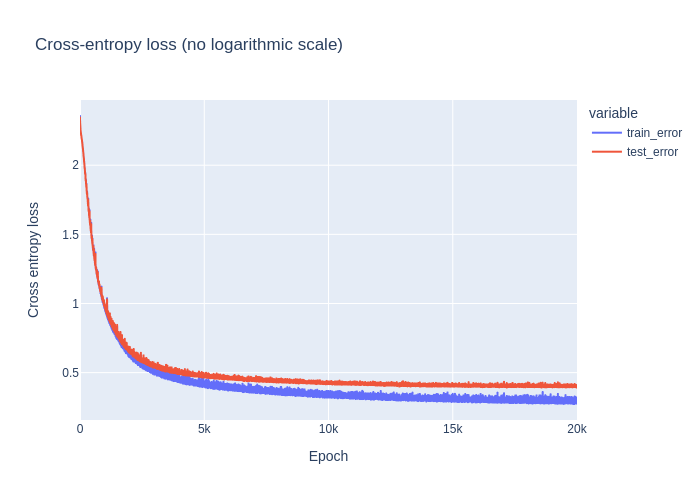
\includegraphics[width=0.8\textwidth]{images/cross-entropy-comparison-2-10-10.png}
    \caption{Comparison of cross entropy loss between train and test dataset with linear scale (architecture $2 \times 10$ fully-connected).}
\end{figure}
\begin{figure}[ht]
    \centering
    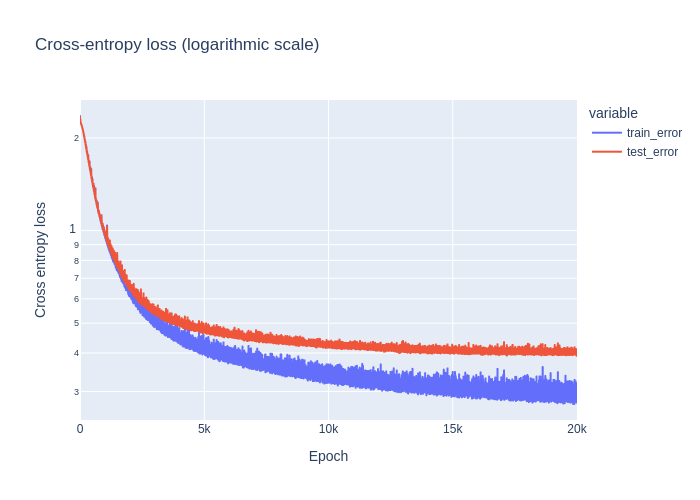
\includegraphics[width=0.8\textwidth]{images/cross-entropy-comparison-2-10-10-log.png}
    \caption{Comparison of cross entropy loss between train and test dataset with log scale (architecture $2 \times 10$ fully-connected).}
\end{figure}
\subsection{Question 3}
\subsection{Question 4}
\subsection{Question 5}
\subsection{Question 6}
\subsection{Question 7}

\end{document}